\chapter{一元函数微分学}

在工程技术或对物理的研究中,通常要知道一个运动的趋势,能不能达到某一点,变化过程是否均匀,趋向什么状态等。
要解决这类问题,需要对函数的变化和趋势进行研究,导数和微分就是解决这类问题的工具。

从微积分的两个对立概念“微分”和“积分”来看,微分是从变化的角度考察函数,积分是从累积的角度考察函数。

对于导数:
\begin{itemize}
    \item 充分理解其数学定义、几何意义和物理意义。
    \item 熟练掌握导数基本公式、复合函数、隐函数和参数式函数的求导方法。
    \item 掌握洛必达法则,学会用该法则求解不定型的极限。
    \item 学会推导三个基本导数公式。
    \item 理解和掌握麦克劳林公式,学会用麦克劳林公式将超越方程转化为多项式方程求解工程问题。
\end{itemize}

对于微分:
\begin{itemize}
    \item 充分理解微分的数学定义、几何意义和物理意义。
    \item 理解微分和导数的关系,并能证明微分定理。
    \item 学会使用微分求解工程上的近似问题。
\end{itemize}

\newpage
\section{光滑曲线的第二个要求}

上一章讨论了光滑的第一个要求——不断,本章讨论我们定义光滑的第二个要求——不折。
如下曲线,在$x_0$处折了。

\begin{figure}[h]
\centering
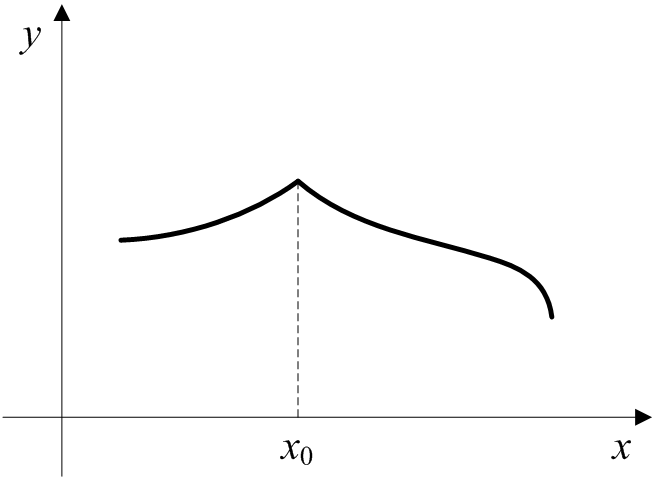
\includegraphics[height=4cm]{2.1.png}
\end{figure}






\newpage
\section{导数}

本节给出导数的概念。
着重理解导数,并使用概念证明函数的可导性。

本节要点:
\begin{itemize}
    \item 理解导数概念;
    \item 熟练掌握初等函数的导数公式表;
    \item 掌握四类函数(复合函数、反函数、隐函数、参数式函数)的求导方法。
\end{itemize}

%============================================================
\subsection{导数的概念}

\begin{definition}[增量]
函数表示了两个变量(自变量和因变量)之间的关系。我们定义,{\bf 自变量的增量}是两个自变量的差,{\bf 因变量的增量}是两个因变量的差,即:
\begin{align*}
&\Delta x:=x_1-x_0 \\
&\Delta y:=y_1-y_0=f\left( x_1 \right) -f\left( x_0 \right)
\end{align*}
\end{definition}

\begin{definition}[变化率]
我们定义两个增量的比值为{\bf 函数的变化率},即:
\[
\frac{\Delta y}{\Delta x}=\frac{f\left( x_1 \right) -f\left( x_0 \right)}{x_1-x_0}=\frac{f\left( x_0+\Delta x \right) -f\left( x_0 \right)}{\Delta x}
\]
\end{definition}

显然,函数的变化率是一个和自变量及其增量区间有关的新函数。
当取相同的$\Delta x$时,变化率描述了函数的变化快慢。
变化率越大,说明函数在同等$\Delta x$下的变化越大。

下面我们考察函数在一个点上的变化率,即当$x_1\rightarrow x_0$(或$\Delta x\rightarrow 0$),函数的变化率的存在性和取值。

\begin{definition}[导数]
设函数$f\left( x \right) $在点$x_0$的某邻域$N\left( x_0 \right) $内有定义,若当$\Delta x\rightarrow 0$时$\Delta y/\Delta x$的极限存在,则称{\bf 函数$f\left( x \right) $在$x_0$处可导},并称此极限值为{\bf 函数$f\left( x \right) $在点$x_0$的导数(derivative)},记为$f'\left( x_0 \right) $,即:
\[
f'\left( x_0 \right) :=\underset{\Delta x\rightarrow 0}{\lim}\frac{\Delta y}{\Delta x} \quad \text{或} \quad f'\left( x_0 \right) :=\underset{x_1\rightarrow x_0}{\lim}\frac{f\left( x_1 \right) -f\left( x_0 \right)}{x_1-x_0}
\]
也可用莱布尼兹(Leibniz)记号记为:
\[
\left. y' \right|_{x=x_0} \quad \text{或} \quad \left. \frac{dy}{dx} \right|_{x=x_0}
\]
\end{definition}

从定义上来讲,函数$f\left( x \right) $在$x_0$处的导数是一个极限,是一个可计算的确定的数。

\begin{definition}[左导数]
设函数$f\left( x \right) $在点$x_0$的左邻域$\left( x_0-\delta ,x_0 \right) $内有定义,若当$\Delta x\rightarrow 0^-$时$\Delta y/\Delta x$的极限存在,则称{\bf 函数$f\left( x \right) $在点$x_0$处左可导},并称此极限值为{\bf 函数$f\left( x \right) $在点$x_0$处的左导数},记为$f'_-\left( x_0 \right) $,即:
\[
f'_-\left( x_0 \right) :=\underset{\Delta x\rightarrow 0^-}{\lim}\frac{\Delta y}{\Delta x}=\underset{x_1\rightarrow {x_0}^-}{\lim}\frac{f\left( x_1 \right) -f\left( x_0 \right)}{x_1-x_0}
\]
\end{definition}

\begin{definition}[右导数]
设函数$f\left( x \right) $在点$x_0$的右邻域$\left( x_0,x_0+\delta \right) $内有定义,若当$\Delta x\rightarrow 0^+$时$\Delta y/\Delta x$的极限存在,则称{\bf 函数$f\left( x \right) $在点$x_0$处右可导},并称此极限值为{\bf 函数$f\left( x \right) $在点$x_0$处的右导数},记为$f'_+\left( x_0 \right) $,即:
\[
f'_+\left( x_0 \right) :=\underset{\Delta x\rightarrow 0^+}{\lim}\frac{\Delta y}{\Delta x}=\underset{x_1\rightarrow {x_0}^+}{\lim}\frac{f\left( x_1 \right) -f\left( x_0 \right)}{x_1-x_0}
\]
\end{definition}

\begin{definition}[导函数]
如果函数$f\left( x \right) $在区间$D$内每一点都可导,则称每个导数构成的新函数为{\bf $f\left( x \right) $的导函数},记为$f'\left( x \right) $(或$y'$)。
显然,导函数$f'\left( x \right) $在$x_0$的值就是导数$f'\left( x_0 \right) $。
\end{definition}

除非特别指明,一般我们将导函数简称为导数。
区间$\left( a,b \right) $(或$\left[ a,b \right] $)内所有可导函数的集合通常记作$D\left( a,b \right) $(或$D\left[ a,b \right] $),所以$f\left( x \right) $在区间$D$内可导也可记作$f\left( x \right) \in D\left( a,b \right) $(或$f\left( x \right) \in D\left[ a,b \right] $)。

求导是对函数的一种运算。
运算对象是函数,得到的结果是另一个函数。
从集合角度,求导是一个函数集合到另一个函数集合的映射。

\begin{tcolorbox}
在讨论导数的时候,紧紧抓住导数的定义,从定义出发。
后续关于导数的定理和公式都是用定义证明和推导。
\end{tcolorbox}

%============================================================
\subsection{导数的几何意义}

考察如下曲线。
\begin{figure}[h]
\centering
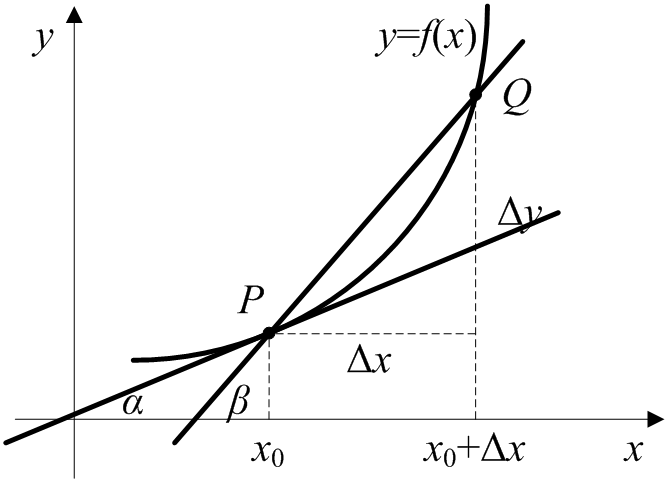
\includegraphics[height=4cm]{2.2.png}
\end{figure}

函数在{\it PQ}之间的变化率在几何上体现为割线{\it PQ}的斜率:
\[
\tan \beta =\frac{\Delta y}{\Delta x}
\]
函数在{\it P}点上的变化率在几何上体现为曲线在{\it P}点处的切线的斜率:
\[
\tan \alpha =\underset{\Delta x\rightarrow 0}{\lim}\frac{\Delta y}{\Delta x}=f'\left( x_0 \right)
\]
如果曲线沿着左右两个方向靠近{\it P}点时的切线斜率是一样的,就说明该点不折。
再看本章一开始的曲线,该曲线在$x_0$处左右导数都是有的,但不相等。
\begin{figure}[ht]
\centering
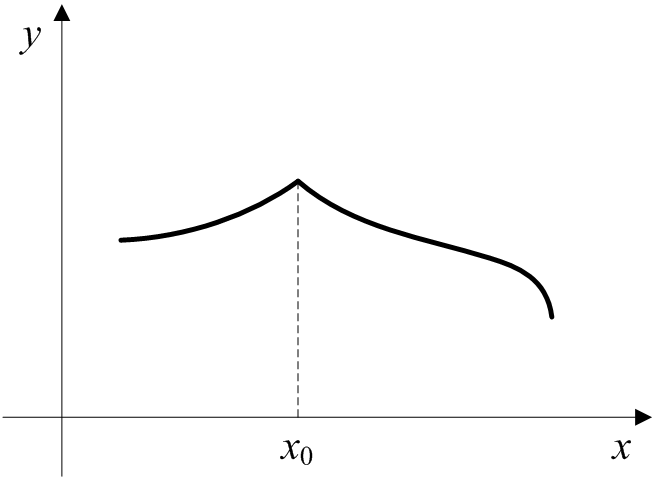
\includegraphics[height=4cm]{2.1.png}
\end{figure}

从几何上来讲,导数的意义是切线的斜率。
反映到光滑上,导数给出了对光滑的第二要求“不折”的数学定义。

%============================================================
\subsection{曲线的切线和法线}

我们将导数这个工具应用到曲线的分析上,分析曲线上任意一点处的切线和法线。

曲线在代数上可以定义为函数$y=f\left( x \right) ,x\in D$。现在我们已知曲线上任何一点$\left( x_0,y_0 \right) $处的斜率就是该点处的导数$f'\left( x_0 \right) $,于是我们得到了曲线上任意一点处的切线和法线的粗略的表达式:
\begin{align*}
&y_{tangent}=f'\left( x_0 \right) x+c \\
&y_{normal}=-\frac{1}{f'\left( x_0 \right)}x+c
\end{align*}
将点$\left( x_0,y_0 \right) $带入即可求得$c$,最终得到切线和法线方程如下:
\begin{align*}
&y_{tangent}=f'\left( x_0 \right) x+\left[ f\left( x_0 \right) -f'\left( x_0 \right) x_0 \right] \\
&y_{normal}=-\frac{1}{f'\left( x_0 \right)}x+\left[ f\left( x_0 \right) +\frac{1}{f'\left( x_0 \right)}x_0 \right]
\end{align*}

%============================================================
\subsection{导数的物理意义}

物理上,导数描述了一个物理量的瞬时变化速度。
比方说路程的导数是速度,速度的导数是加速度。
导数为求解物理量的变化速度提供了强大的数学工具。

有的时候,我们知道两个物理量之间的关系和其中一个物理量的变化率,通过导数就可以得到另一个物理量的变化率。
实际问题中,前者的变化率已知且简单,后者变化率复杂,无法直接获得,通过这个方法就可以获得一个复杂的、不直观的变化率。
换一种说法,我们要获得一个物理量的变化率,但该变化率复杂,难以通过常规的方法求解。
我们可以将它关联到一个具有简单已知的变化率的物理量,通过导数的运算和求导法则计算得到,比如观测仰角的变化率。

%============================================================
\subsection{导数的定理}

\begin{theorem}
$f\left( x \right) $在$x_0$处可导$\Leftrightarrow f\left( x \right) $在$x_0$处左右导数存在且相等,即$f'_-\left( x_0 \right) =f'_+\left( x_0 \right) $。
\end{theorem}

\begin{theorem}
$f\left( x \right) $在$x_0$处可导$\Leftrightarrow f\left( x \right) $在$x_0$处连续。
\end{theorem}

\begin{proof}
从连续的定义出发,即证明$\underset{x\rightarrow x_0}{\lim}\left[ f\left( x \right) -f\left( x_0 \right) \right] =0$。
\begin{align*}
\underset{x\rightarrow x_0}{\lim}\left[ f\left( x \right) -f\left( x_0 \right) \right] &=\underset{x\rightarrow x_0}{\lim}\frac{f\left( x \right) -f\left( x_0 \right)}{x-x_0}\cdot \left( x-x_0 \right) \\
&=f'\left( x_0 \right) \underset{x\rightarrow x_0}{\lim}\left( x-x_0 \right) =0
\end{align*}
\end{proof}

%============================================================
\subsection{导数的四则运算}

\begin{align*}
&\left( C\cdot f \right) '=C\cdot f' \\
&\left( f\pm g \right) '=f'\pm g' \\
&\left( f\cdot g \right) '=f'g+fg' \\
&\left( \frac{f}{g} \right) '=\frac{f'g-fg'}{g^2} \\
&\left( \frac{1}{g} \right) '=-\frac{g'}{g^2}
\end{align*}

前两个公式表明导数运算是线性的。

%============================================================
\subsection{导数的基本公式}

\begin{align*}
\begin{matrix}
	\left( C \right) '=0 \hfill                                       & \left( x^a \right) '=a\cdot x^{a-1} \hfill \\
	\left( a^x \right) '=a^x\ln a \hfill                              & \left( e^x \right) '=e^x \hfill \\
	\left( \log _ax \right) '=\frac{1}{x\ln a} \hfill                 & \left( \ln x \right) '=\frac{1}{x} \hfill \\
	\left( \sin x \right) '=\cos x \hfill                             & \left( \cos x \right) '=-\sin x \hfill \\
	\left( \tan x \right) '=\sec ^2x \hfill                           & \left( \cot x \right) '=-\csc ^2x \hfill \\
	\left( \sec x \right) '=\sec x\cdot \tan x \hfill                 & \left( \csc x \right) '=-\csc x\cdot \cot x \hfill \\
	\left( \mathrm{arc}\sin x \right) '=\frac{1}{\sqrt{1-x^2}} \hfill & \left( \mathrm{arc}\cos x \right) '=-\frac{1}{\sqrt{1-x^2}} \hfill \\
	\left( \mathrm{arc}\tan x \right) '=\frac{1}{1+x^2} \hfill        & \left( \mathrm{arc}\cot x \right) '=-\frac{1}{1+x^2} \hfill \\
	\left( \mathrm{sh}x \right) '=\mathrm{ch}x \hfill                 & \left( \mathrm{ch}x \right) '=\mathrm{sh}x \hfill \\
\end{matrix}
\end{align*}

以上基本公式中,除了$\left( C \right) ',\left( a^x \right) ',\left( \sin x \right) '$,其余都可以从这三个公式导出。

{\bf 计算$\left( C \right) '$}
\[
\left( C \right) '=\underset{\Delta x\rightarrow 0}{\lim}\frac{C-C}{\Delta x}=0
\]

{\bf 计算$\left( a^x \right) '$}
\[
\left( a^x \right) '=\underset{\Delta x\rightarrow 0}{\lim}\frac{a^{x+\Delta x}-a^x}{\Delta x}=a^x\underset{\Delta x\rightarrow 0}{\lim}\frac{a^{\Delta x}-1}{\Delta x}=a^x\ln a
\]

{\bf 计算$\left( \sin x \right) '$}
\begin{align*}
\left( \sin x \right) '&=\underset{\Delta x\rightarrow 0}{\lim}\frac{\sin \left( x+\Delta x \right) -\sin x}{\Delta x} \\
&=\underset{\Delta x\rightarrow 0}{\lim}\frac{2\sin \frac{\Delta x}{2}\cos \frac{2x+\Delta x}{2}}{\Delta x}=\underset{\Delta x\rightarrow 0}{\lim}cos \frac{2x+\Delta x}{2}=\cos x
\end{align*}

%============================================================
\subsection{复合函数的求导}

\begin{theorem}[复合函数求导定理]
若函数$y=y\left( u \right) ,u=u\left( x \right) $在对应区间可导,则复合函数$y=y\left[ u\left( x \right) \right] $在对应区间也可导,且有:
\[
\frac{dy}{dx}=\frac{dy}{du}\cdot \frac{du}{dx}
\]
\end{theorem}

复合求导法则是接下去三种求导法则(反函数求导、隐函数求导、参数式函数求导)的基础。

%============================================================
\subsection{反函数的求导}

\begin{theorem}[反函数求导定理]
若函数$y=f\left( x \right) $在某区间内单调可导,且$y'\ne 0$,则它的反函数$x=f^{-1}\left( y \right) $在对应区间内也可导,且有:
\[
f'\left( x \right) =\frac{1}{\left( f^{-1} \right) '\left( y \right)}
\]
或写成:
\[
\frac{dy}{dx}=\frac{1}{\frac{dx}{dy}}
\]
\end{theorem}

\begin{proof}
\[
f'\left( x \right) =\underset{\Delta x\rightarrow 0}{\lim}\frac{\Delta y}{\Delta x}=\underset{\Delta x\rightarrow 0}{\lim}\frac{1}{\frac{\Delta x}{\Delta y}}=\frac{1}{\underset{\Delta y\rightarrow 0}{\lim}\frac{\Delta x}{\Delta y}}=\frac{1}{\left( f^{-1} \right) '\left( y \right)}
\]
\end{proof}

~

\begin{example}
设$y=\mathrm{arc}\sin x$,求$y'$。
\end{example}

解:

\[
\frac{dy}{dx}=\frac{1}{\frac{dx}{dy}}=\frac{1}{\left( \sin y \right) '}=\frac{1}{\cos y}=\frac{1}{\sqrt{1-\sin ^2y}}=\frac{1}{\sqrt{1-x^2}}
\]

%============================================================
\subsection{隐函数的求导}

\begin{theorem}[一元隐函数求导定理]
若方程$F\left( x,y \right) =0$确定唯一的单值连续可导函数$y=f\left( x \right) $,则有:
\[
\frac{dy}{dx}=-\frac{F_x}{F_y}
\]
其中:
\begin{itemize}
	\item $F_x$:表示$F\left( x,y \right) =0$对$x$求导,$x$是自变量,$y$是常量;
	\item $F_y$:表示$F\left( x,y \right) =0$对$y$求导,$y$是自变量,$x$是常量。
\end{itemize}
\end{theorem}


\begin{tcolorbox}
该定理在多元函数微积分中证明,这里只需知道如何计算一元隐函数的导数。
\end{tcolorbox}

~

\begin{example}
假设方程$e^y=e-xy$确定了函数$y=f\left( x \right) $,求$y'$。
\end{example}

解:

令$F\left( x,y \right) :=e^y-e+xy=0$,得:
\begin{align*}
&\because \begin{cases}
	F_x=y\\
	F_y=e^y+x\\
\end{cases} \\
&\therefore y'=-\frac{F_x}{F_y}=-\frac{y}{e^y+x}
\end{align*}

%============================================================
\subsection{参数式函数的求导}

\begin{theorem}[参数函数求导定理]
若参数方程
\begin{align*}
\begin{cases}
	x=x\left( t \right)\\
	y=y\left( t \right)\\
\end{cases}
\end{align*}
可导,$x=x\left( t \right) $存在可导的反函数,且$x'\left( t \right) \ne 0$,则由该参数方程确定的函数$y=f\left( x \right) $可导,且有:
\[
\frac{dy}{dx}=\frac{y'\left( t \right)}{x'\left( t \right)}
\]
\end{theorem}

~

\begin{example}
若有摆线
\begin{align*}
\begin{cases}
	x=t-\sin t\\
	y=1-\cos t\\
\end{cases}
\end{align*}
求$t=\pi /2$处的切线方程。
\end{example}

解:

切线方程$y=f'\left( x_0 \right) x+\left[ f\left( x_0 \right) -f'\left( x_0 \right) x_0 \right] $,可得:
\begin{align*}
&\left. \frac{dy}{dx} \right|_{t=\pi /2}=\left. \frac{dy}{dt}/\frac{dx}{dt} \right|_{t=\pi /2}=\left. \frac{\sin t}{1-\cos t} \right|_{t=\pi /2}=1 \\
&y=1\cdot x+\left[ \left( 1-\cos \frac{\pi}{2} \right) -1\cdot \left( \frac{\pi}{2}-1 \right) \right] =x+2-\frac{\pi}{2}
\end{align*}

%============================================================
\subsection{高阶导数}

\begin{definition}[二阶导数]
设函数$f\left( x \right) $在点$x_0$的某邻域$N\left( x_0 \right) $内可导,若极限
\[
\underset{\Delta x\rightarrow 0}{\lim}\frac{f'\left( x_0+\Delta x \right) -f'\left( x_0 \right)}{\Delta x}
\]
存在,则称该极限值为{\bf $f\left( x \right) $在点$x_0$处的二阶导数},记作:
\[
f''\left( x_0 \right) \quad \text{或} \quad \left. y'' \right|_{x=x_0} \quad \text{或} \quad \left. \frac{d^2y}{dx^2} \right|_{x=x_0}
\]
\end{definition}

同样,我们可以定义三阶导数、四阶导数、直至n阶导数。






\newpage
\section{微分}

本节给出微分概念。
着重理解微分及其意义和工程应用。

本节要点:
\begin{itemize}
    \item 熟练掌握微分概念;
    \item 学会推导微分定理。
\end{itemize}

~

工程上,经常碰到已知$f\left( x_0 \right) $,求$f\left( x_0+\Delta x \right) $的问题。
这个问题在数学上就是$\Delta y$能不能通过$\Delta x$的线性计算获得,误差多少,即:
\[
\Delta y=A\Delta x+B\left( \Delta x \right)
\]
且我们希望$A$与$\Delta x$无关,$B\left( \Delta x \right) $与$\Delta x$有关。

考虑这么几个问题:
\begin{itemize}
    \item 这个表达式能不能成立;
    \item $A$的值是多少;
    \item $B\left( \Delta x \right) $能不能忽略,什么时候可以忽略。
\end{itemize}

%============================================================
\subsection{微分的概念}

\begin{definition}[微分]
设函数$f\left( x \right) $在点$x_0$的某邻域$N\left( x_0 \right) $内有定义,若自变量增量$\Delta x$和因变量增量$\Delta y$满足:
\[
\Delta y=A\left( x_0 \right) \Delta x+o\left( \Delta x \right)
\]
其中:
\begin{itemize}
    \item $A\left( x_0 \right) $:一个只与$x_0$有关,与$\Delta x$无关的量,
    \item $o\left( \Delta x \right) $:一个当$\Delta x\rightarrow 0$时的高阶无穷小量,
\end{itemize}
则称{\bf 函数$f\left( x \right) $在点$x_0$处可微},$A\left( x_0 \right) \Delta x$称为{\bf 函数在点$x_0$处的微分(differentials)}(也称为$\Delta y$的{\bf 线性主部}),记为$dy$,即
\[
dy:=A\left( x_0 \right) \Delta x
\]
\end{definition}

微分表达的意思是,如果增量$\Delta y$中可以忽略一个误差$o\left( \Delta x \right) $而剩下一个线性部分,则增量可以用一个“微增量$dy$”代替,即:
\[
\Delta y=dy+o\left( \Delta x \right) \approx dy
\]
几何上,微分表达的就是“光滑”。
一个函数在某点可微,必须在该点是不断的、不折的。
充分理解这点,可微和可导的关系也就自然而然了。

%============================================================
\subsection{微分的运算法则}

微分的运算四则法则,包括复合函数、隐函数、反函数的微分法则,同导数,不细展开。

~

\begin{example}
若$3x^2y^3+xy+x^2=0$确定函数$y=\left( x \right) $,求$dy$。
\end{example}

解:
\begin{align*}
&\because \frac{dy}{dx}=-\frac{F_x}{F_y}=\frac{3y^3\cdot 2x+y+2x}{3x^2\cdot 3y^2+x}=-\frac{6xy^3+2x+y}{9x^2y^2+x} \\
&\therefore dy=\frac{6xy^3+2x+y}{9x^2y^2+x}\cdot dx
\end{align*}

%============================================================
\subsection{微分和导数的关系}

\begin{theorem}[微分定理]
$y=f\left( x \right) $在点$x_0$处可微$\Leftrightarrow y=f\left( x \right) $在点$x_0$处可导,且$A\left( x_0 \right) =f'\left( x_0 \right) $。
\end{theorem}

\begin{proof}
即计算$f'\left( x_0 \right) $。
从导数的定义出发,如果可微,有$\Delta y=A\left( x_0 \right) \Delta x+o\left( \Delta x \right) $,则:
\[
f'\left( x_0 \right) =\underset{\Delta x\rightarrow 0}{\lim}\frac{\Delta y}{\Delta x}=\underset{\Delta x\rightarrow 0}{\lim}\frac{A\left( x_0 \right) \Delta x+o\left( \Delta x \right)}{\Delta x}=A\left( x_0 \right)
\]
\end{proof}

如果$y=f\left( x \right) $在区间内每一点都可微,则称函数在区间内可微。
由于$\Delta x=dx$,于是微分表达式又可以写作:
\[
dy=A\left( x \right) dx=f'\left( x \right) dx
\]
或者写成微商的形式:
\[
\frac{dy}{dx}=A\left( x \right) =f'\left( x \right)
\]

导数$y'$是描述函数的变化率,微分$dy$是描述近似量。
从概念上讲,是有区别的。
\[
y'=\underset{\Delta x\rightarrow 0}{\lim}\frac{\Delta y}{\Delta x} \qquad dy=\underset{\Delta x\rightarrow 0}{\lim}\Delta y
\]
微分定理将导数和微分两个概念联系起来,揭示出两者之间的关系:
\[
dy=y'\cdot dx
\]
所以,不要把$y'$和$\frac{dy}{dx}$看成一个概念,更不要把$\frac{dy}{dx}$看成一个记号。
前者是变化率,几何上是切线斜率,后者是两个微分的比。

%============================================================
\subsection{微分的几何意义}

如下图,$\Delta y$是线段{\it MQ}的长度,且$\Delta y=\tan \beta \cdot \Delta x$,也是因变量的正真的增量。
$dy$是线段{\it MN}的长度,且$dy=\tan \alpha \cdot \Delta x$。
它们之间差了线段{\it NQ}。

\begin{figure}[h]
\centering
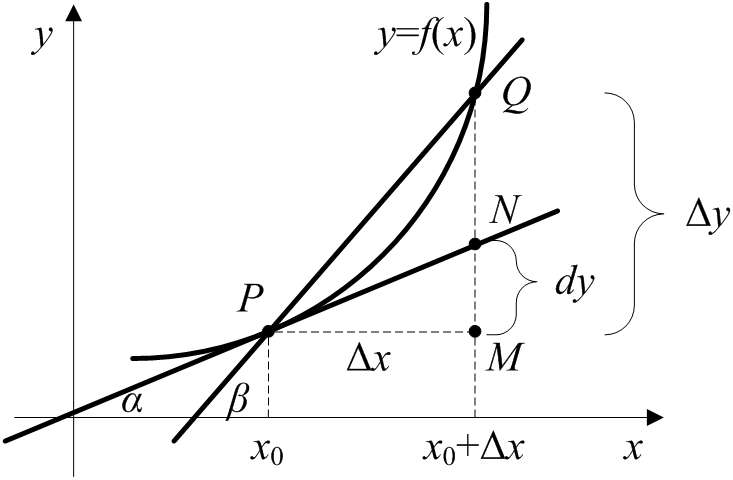
\includegraphics[height=4cm]{2.3.png}
\end{figure}

当{\it Q}点无穷逼近{\it P}的时候,即$\beta \rightarrow \alpha $,可得:
\[
\underset{\Delta x\rightarrow 0}{\lim}\Delta y=\underset{\Delta x\rightarrow 0}{\lim}\left( \tan \beta \cdot \Delta x \right) =\tan \alpha \cdot \Delta x=dy
\]
从几何上看,当{\it Q}点无穷逼近{\it P}的时候,线段{\it MQ}的长度无穷逼近线段{\it MN}的长度。
或者说,我们可以用线段{\it MQ}代替线段{\it MN},且线段{\it NQ}是可以被忽略的。
被忽略的{\it NQ}就是那个高阶无穷小量$o\left( \Delta x \right) $。

微分的几何意义是在一个微小的局部,我们可以用直线函数近似代替曲线函数,即“以直代曲”。
这种局部线性化的思想广泛应用于自然科学和工程。

%============================================================
\subsection{微分的物理应用}

用微分我们可以近似计算一些工程值。
若已知$f\left( x_0 \right) $,如何快速求$f\left( x_0+\Delta x \right) $处的值。
这类问题可以通过微分近似求解。当$\Delta x$足够小时,我们可以用$dy$代替$\Delta y$,从而有:
\[
y=f\left( x_0 \right) +\Delta y\approx f\left( x_0 \right) +dy
\]

~

\begin{example}
扩音器插头为一圆柱体,截面半径r=0.15cm,长l=4cm,为提高导电性,需要在该圆柱体侧面镀一层0.001cm的纯铜,问约需要多少。
\end{example}

解:

显然该问题就是估算体积的变化。
圆柱体体积:
\[
V=\pi r^2l
\]
侧面镀一层纯铜,相当于半径变化。
所用铜的体积等于由于半径的微小变化引起的圆柱体体积的微增量。
\[
dV=2\pi rl=2\pi \cdot 0.15\cdot 4\cdot 0.001=0.00377\mathrm{cm}^3
\]






\newpage
\section{导数的应用}

导数是描述一个函数的变化率,所以通过导数我们可以分析一个函数的变化趋势、形态、走向,进而用多项式近似该函数。
微分中值定理解决前者,泰勒展开和麦克劳林公式解决后者。

本节要点:
\begin{itemize}
    \item 掌握各个定理。
\end{itemize}

%============================================================
\subsection{微分中值定理}

\begin{theorem}[费马定理]
设$f\left( x \right) $在点$x_0$处可导,若$x_0$处是$f\left( x \right) $的一个极值点,则$f'\left( x_0 \right) =0$。
\end{theorem}

\begin{theorem}[罗尔定理]
设$f\left( x \right) $在$\left[ a,b \right] $连续,在$\left( a,b \right) $可导,若$f\left( a \right) =f\left( b \right) $,则必有$\xi \in \left( a,b \right) $,使得$f'\left( \xi \right) =0$。
即两端相等的光滑曲线必有极值点。
\end{theorem}

\begin{theorem}[拉格朗日定理]
设$f\left( x \right) $在$\left[ a,b \right] $连续,在$\left( a,b \right) $可导,则必有$\xi \in \left( a,b \right) $,使得$f'\left( \xi \right) =\frac{f\left( b \right) -f\left( a \right)}{b-a}$。
即可作切线和割线平行。
\end{theorem}

\begin{theorem}[柯西定理]
设$f\left( x \right) $在$\left[ a,b \right] $连续,在$\left( a,b \right) $可导,若$g'\left( x_0 \right) \ne 0$,则必有$\xi \in \left( a,b \right) $,使得$\frac{f'\left( \xi \right)}{g'\left( \xi \right)}=\frac{f\left( b \right) -f\left( a \right)}{g\left( b \right) -g\left( a \right)}$。
\end{theorem}

微分中值定理建立了函数在考察区间内的变化形态。
这四个微分中值定理,前提都是要求可导,说明被考察对象都是光滑曲线。
而光滑,则直觉上必然会有这些定理描述的现象。
充分理解光滑的含义,这些定理也将是不证自明。

费马定理可用于求解区间内的最大值最小值问题。

罗尔定理可用于判断一个方程有无根,考察它的原函数在区间内连续可导,如果区间端点值相等,则必有根。

拉格朗日定理和后面的积分中值定理是对应关系,以不同的角度描述了一个事情,一个从微分角度,一个从积分角度。

柯西定理是拉格朗日定理的推广。

%============================================================
\subsection{洛必达法则}

\begin{theorem}[洛必达法则(L'Hopital's rule)]
若$f\left( x \right) ,g\left( x \right) $满足:
\begin{itemize}
    \item $\underset{x\rightarrow x_0}{\lim}f\left( x \right) =0,\underset{x\rightarrow x_0}{\lim}g\left( x \right) =0$;
    \item 在点$x_0$的去心邻域内$f'\left( x \right) ,g'\left( x \right) $均存在,且$g'\left( x \right) \ne 0$;
    \item $\underset{x\rightarrow x_0}{\lim}\frac{f'\left( x \right)}{g'\left( x \right)}$存在(或为$\infty $);
\end{itemize}
则有:
\[
\underset{x\rightarrow x_0}{\lim}\frac{f\left( x \right)}{g\left( x \right)}=\underset{x\rightarrow x_0}{\lim}\frac{f'\left( x \right)}{g'\left( x \right)}
\]
\end{theorem}

洛必达法则用于求解$\frac{0}{0}$和$\frac{\infty}{\infty}$之类的不定型极限。
注意,其他类型的极限不能用洛必达法则。






\newpage
\section{泰勒展开}

\begin{tcolorbox}
从逻辑概念的归属来讲,泰勒定理属于级数的范畴,应该和三角级数编排在一起。
而从三角级数到傅里叶变换需要一点多元函数积分的概念,所以泰勒展开会在级数部分详细介绍。
但如果把泰勒展开完全编排在最后,等学完所有的微积分内容(特别是多元函数微积分)再学级数,那对很多工程应用来说就学了一堆不需要的东西(电子电路就不需要多元函数微积分的概念),而且大大增加学习难度。
所以一般教材的编排将泰勒定理放在这里讲述。
\end{tcolorbox}

本节讨论导数一个很重要、很典型的应用——多项式展开。

本节要点:
\begin{itemize}
    \item 掌握泰勒展开的概念;
    \item 从线性代数角度理解泰勒展开;
    \item 掌握麦克劳林公式;
    \item 熟悉泰勒展开的工程使用。
\end{itemize}

%============================================================
\subsection{泰勒定理}

之前在讨论微分时,我们将任意可导函数$f\left( x_0 \right) $在$x_0$的一个微小局部用一个线性表达式$f\left( x \right) \approx f\left( x_0 \right) +f'\left( x_0 \right) \left( x-x_0 \right) $描述。
进一步地,我们希望在$x_0$附近找到一个关于$x$的多项式$P\left( x \right) $,能够表示$x\left( x \right) $,要求很简单:
\begin{itemize}
    \item $P\left( x \right) $和$x\left( x \right) $在$x_0$有相同的函数值和1~n阶导数;
    \item $P\left( x \right) $和$x\left( x \right) $的误差能定量描述。
\end{itemize}

~

\begin{theorem}[泰勒(Taylor)定理]
若$f\left( x \right) $在$x_0$处满足n阶可导,则$f\left( x \right) $可以展开成:
\begin{align*}
f\left( x \right) &=f\left( x_0 \right) +f'\left( x_0 \right) \left( x-x_0 \right) +\frac{f''\left( x_0 \right)}{2!}\left( x-x_0 \right) ^2+\cdots \\
&\quad +\frac{f^{\left( n \right)}\left( x_0 \right)}{n!}\left( x-x_0 \right) ^n+o\left( \left( x-x_0 \right) ^n \right) \\
&=\left[ \sum_{i=0}^n{\frac{f^{\left( i \right)}\left( x_0 \right)}{i!}\left( x-x_0 \right) ^i} \right] +o\left( \left( x-x_0 \right) ^n \right)
\end{align*}
其中$R\left( x \right) :=o\left( \left( x-x_0 \right) ^n \right) $称为{\bf 佩亚诺(G. Peano)型余项}。
\end{theorem}

当$n=1$时,泰勒展开就是一阶微分形式:
\begin{align*}
&\because f\left( x \right) =f\left( x_0 \right) +f'\left( x_0 \right) \left( x-x_0 \right) +o\left( x-x_0 \right) \\
&\therefore \Delta y=f\left( x \right) -f\left( x_0 \right) =f'\left( x_0 \right) \left( x-x_0 \right) +o\left( x-x_0 \right)
\end{align*}

\begin{theorem}[泰勒(Taylor)定理]
若$f\left( x \right) $在区间$D$上满足n+1阶可导,则$\forall x,x_0\in D$,至少存在$\xi \in \left[ x,x_0 \right] $或$\xi \in \left[ x_0,x \right] $,使得:
\begin{align*}
f\left( x \right) &=f\left( x_0 \right) +f'\left( x_0 \right) \left( x-x_0 \right) +\frac{f''\left( x_0 \right)}{2!}\left( x-x_0 \right) ^2+\cdots \\
&\quad +\frac{f^{\left( n \right)}\left( x_0 \right)}{n!}\left( x-x_0 \right) ^n+\frac{f^{\left( n+1 \right)}\left( \xi \right)}{\left( n+1 \right) !}\left( x-x_0 \right) ^{n+1} \\
&=\left[ \sum_{i=0}^n{\frac{f^{\left( i \right)}\left( x_0 \right)}{i!}\left( x-x_0 \right) ^i} \right] +\frac{f^{\left( n+1 \right)}\left( \xi \right)}{\left( n+1 \right) !}\left( x-x_0 \right) ^{n+1}
\end{align*}
其中$R_n\left( x \right) :=\frac{f^{\left( n+1 \right)}\left( \xi \right)}{\left( n+1 \right) !}\left( x-x_0 \right) ^{n+1}$称为{\bf 朗格兰日(Lagrange)型余项}。
\end{theorem}

泰勒定理告诉我们,任何n阶可导函数,都可以展开成一个二项式。
虽然两个都是泰勒定理,但第二个泰勒定理的要求更严格,好处是给出了余项的表达式,可以用来估算误差。
泰勒定理其实就是一个函数的幂级数展开。

%============================================================
\subsection{从线性代数看泰勒展开}

从线性代数角度看来,泰勒展开就将函数将基变换为多项式。
原来$f\left( x \right) $的基为实数集$D$,变换后为:
\[
B=\left[ \begin{array}{c}
	1\\
	\left( x-x_0 \right)\\
	\left( x-x_0 \right) ^2\\
	\vdots\\
	\left( x-x_0 \right) ^n\\
\end{array} \right]
\]
相应地坐标为:
\[
\left[ f \right] _B=\left[ \begin{array}{c}
	f\left( x_0 \right)\\
	f'\left( x_0 \right)\\
	\frac{f''\left( x_0 \right)}{2!}\\
	\vdots\\
	\frac{f^{\left( n \right)}\left( x_0 \right)}{n!}\\
\end{array} \right]
\]
于是函数可以描述为:
\[
f\left( x \right) =B^T\left[ f \right] _B+R_n\left( x \right)
\]

%============================================================
\subsection{麦克劳林公式}

\begin{definition}[n阶麦克劳林(Maclaurin)公式]
{\bf 麦克劳林公式}是函数在0点处的泰勒展开,取$x_0=0$,泰勒展开公式变为:
\begin{align*}
f\left( x \right) &=f\left( 0 \right) +f'\left( 0 \right) \cdot x+\frac{f''\left( 0 \right)}{2!}\cdot x^2+\cdots +\frac{f^{\left( n \right)}\left( 0 \right)}{n!}\cdot x^n+o\left( x \right) \\
&=\left[ \sum_{i=0}^n{\frac{f^{\left( i \right)}\left( 0 \right)}{i!}\cdot x^i} \right] +o\left( x \right)
\end{align*}
\end{definition}

~

几个常用函数的麦克劳林公式:
\begin{align*}
&\left( 1+x \right) ^a=1+ax+\frac{a\left( a-1 \right)}{2!}x^2+\cdots +\frac{a\left( a-1 \right) \cdots \left( a-n \right)}{n!}x^n+o\left( x \right) \\
&e^x=1+x+\frac{x^2}{2!}+\cdots +\frac{x^n}{n!}+o\left( x \right) \\
&\sin x=x-\frac{x^3}{3!}+\frac{x^5}{5!}-\cdots +\left( -1 \right) ^{m-1}\frac{x^{2m-1}}{\left( 2m-1 \right) !}+o\left( x \right) \\
&\cos x=1-\frac{x^2}{2!}+\frac{x^4}{4!}-\cdots +\left( -1 \right) ^m\frac{x^{2m}}{\left( 2m \right) !}+o\left( x \right)
\end{align*}

特别地,一般在工程中常用:
\begin{align*}
&\left( 1+x \right) ^a=1+ax \\
&e^x=1+x \\
&\sin x=x \\
&\cos x=1-\frac{x^2}{2!}
\end{align*}

麦克劳林公式常用于工程上的公式推导,通过麦克劳林公式将超越方程简化成一次或二次方程,进而求解解析式。
如求解方程$e^x=\cos x-1$,在0附近可以用方程$1+x=-x^2/2!$代替求解。

%============================================================
\subsection{泰勒展开的工程意义}

要估算一个复杂的函数,通常的做法是用另一个简单的函数代替,即“化繁为简”。
这种方法(或思想)称为级数。
代替的函数必须简单,最好是初等函数的组合。
数学上有三种可行的初等函数代替展开:
\begin{itemize}
    \item 幂函数;
    \item 三角函数;
    \item 指数函数。
\end{itemize}
但由于欧拉公式,所以实际只剩下幂函数和三角函数两种方法。

幂函数展开的方法之一就是泰勒展开,三角函数展开就是傅里叶级数。
泰勒展开由于采用幂函数将超越方程化为二次方程,所以多用于手解超越方程或判断两个超越方程的大小关系。
傅里叶级数采用三角函数,使得原函数由一系列不同角频的正弦函数组成,所以通常用于考察一个函数的特征。






\newpage
\section{函数的性状}

本节我们用导数这个数学工具考察函数的性状。

本节要点:
\begin{itemize}
    \item 掌握函数单调性的判断;
    \item 掌握函数极值的判断;
    \item 掌握目标函数的优化步骤;
    \item 了解凸函数的概念;
    \item 了解琴声Jensen不等式和渐近线。
\end{itemize}

%============================================================
\subsection{单调性}

\begin{theorem}
若$f\left( x \right) \in D\left( a,b \right) $,则:
\begin{itemize}
    \item $f'\left( x \right) \geqslant 0\left( \leqslant 0 \right) \Leftrightarrow f\left( x \right) $在$\left( a,b \right) $上单调增(减);
    \item $f'\left( x \right) >0\left( <0 \right) \Leftrightarrow f\left( x \right) $在$\left( a,b \right) $上严格单调增(减)。
\end{itemize}
\end{theorem}

\begin{corollary}
若$f\left( x \right) \in C\left[ x_0,x \right] \cap D\left( x_0,x \right) $,且$f\left( x_0 \right) =0$,则:
\begin{itemize}
    \item 当$x>x_0$时$f'\left( x \right) >0$,则$f\left( x \right) >0$;
    \item 当$x>x_0$时$f'\left( x \right) <0$,则$f\left( x \right) <0$。
\end{itemize}
\end{corollary}

推论要表达的是当我们知道函数的某个起点和趋势,我们就可以判断函数的在该点后的值域。

%============================================================
\subsection{极值的判断}

微分中值定理中我们初步讨论了极值,这里给出具体的定义和详细讨论。

\begin{definition}[极值和极值点]
设函数$f\left( x \right) $在区间$D$上有定义,若$x_0\in D$存在邻域$N\left( x_0,\delta \right) \subseteq D$,使得$\forall x\in N$有:
\[
f\left( x \right) <f\left( x_0 \right) \quad \text{或} \quad f\left( x \right) >f\left( x_0 \right)
\]
则称$f\left( x_0 \right) $为$f\left( x \right) $在邻域$N$上的一个{\bf 极大值}(或{\bf 极小值},统称为{\bf 极值}),而点$x_0$称为$f\left( x \right) $在邻域$N$上的{\bf 极大值点}(或{\bf 极小值点},统称为{\bf 极值点})。
如果$f\left( x \right) $在区间$D$上可导,则极值点$x_0$处必有$f'\left( x_0 \right) =0$,但$f'\left( x_0 \right) =0$并不代表$x_0$为极值点,我们称$f'\left( x_0 \right) =0$时的$x_0$为$f\left( x_0 \right) =0$的{\bf 驻点}。
如果$f\left( x_0 \right) =0$在$x_0$处不可导,则$x_0$也有可能是极值点。
\end{definition}

\begin{theorem} \label{th_2_6_1}
设$f\left( x \right) =0$在点$x_0$处连续,在$N\left( \hat{x}_0,\delta \right) $内可导,则:
\begin{itemize}
    \item 若$\forall x\in \left( x_0-\delta ,x_0 \right) $有$f'\left( x \right) <0$,$\forall x\in \left( x_0,x_0+\delta \right) $有$f'\left( x \right) >0$,则$f\left( x_0 \right) $为极小值;
    \item 若$\forall x\in \left( x_0-\delta ,x_0 \right) $有$f'\left( x \right) >0$,$\forall x\in \left( x_0,x_0+\delta \right) $有$f'\left( x \right) <0$,则$f\left( x_0 \right) $为极大值;
    \item 若$\forall x\in N\left( \hat{x}_0,\delta \right) $有$f'\left( x \right) $恒为正或恒为负,$f\left( x_0 \right) $为非极值。
\end{itemize}
\end{theorem}

\begin{theorem} \label{th_2_6_2}
设$f\left( x \right) =0$在点$x_0$处存在二阶导数,且$f'\left( x \right) =0$,则:
\begin{itemize}
    \item 若$f''\left( x \right) >0$,则$f\left( x_0 \right) $为极小值;
    \item 若$f''\left( x \right) <0$,则$f\left( x_0 \right) $为极大值;
    \item 若$f''\left( x \right) =0$,不能判定。
\end{itemize}
\end{theorem}

\begin{theorem} \label{th_2_6_3}
设$f\left( x \right) =0$在点$x_0$处存在二阶及以上导数,且
\begin{align*}
&f'\left( x_0 \right) =f''\left( x_0 \right) =\cdots =f^{\left( n-1 \right)}\left( x_0 \right) =0 \\
&f^{\left( n \right)}\left( x_0 \right) \ne 0
\end{align*}
则:
\begin{itemize}
    \item $n$为偶数时,若$f^{\left( n \right)}\left( x_0 \right) >0$则$f\left( x_0 \right) $为极小值,若$f^{\left( n \right)}\left( x_0 \right) <0$则$f\left( x_0 \right) $为极大值;
    \item $n$为奇数时,$f\left( x_0 \right) $非极值。
\end{itemize}
\end{theorem}

上述3个定理是对微分中值定理中的费马定理的推广,费马定理给出的是极值点的必要条件,这里给出了极值的充要条件。
但必须注意,这些定理的前提是可导,不可导点也是潜在的极值点,需要判断。

定理\ref{th_2_6_1}可以从几何上理解,通过描述一阶导数的走势判断极值。
定理\ref{th_2_6_2}通过二阶导数定量化地描述了函数走势,定理证明采用泰勒展开,具体参见“教材\cite{book1}”。
定理\ref{th_2_6_3}是定理\ref{th_2_6_2}的推广。

%============================================================
\subsection{目标函数优化}

极值是一个小范围内的最值,如果将考察区域扩大,则对极值的考察就扩展为对最值的考察。
最值点将会出现在极值点、不可导点和边界点上。
工程上有很多类似考察最值的问题,数学上归结为{\bf 求解目标函数的最值问题},有时又称为{\bf 目标函数的最优化}。

若$f\left( x \right) $在$\left[ a,b \right] $内连续,$\left( a,b \right) $内存在有限个不可导点,则首先根据连续函数的性质,必然存在最值,且两个端点$a,b$、驻点和不可导点$x_i$都是最值可能的点,将这些点的函数值计算就可以判断最值,或者根据一阶导数判断最值。

~

\begin{example}
若$f\left( x \right) =\sqrt[3]{\left( x^2-2x \right) ^2}$,求$\left[ 0,3 \right] $上的最值。
\end{example}

解:

易得$f\left( x \right) $连续,考察一阶导数:
\[
f'\left( x \right) =\frac{4}{3}\frac{x-1}{\sqrt[3]{x^2-2x}}
\]
有$x=1$为驻点,$x=2$为不可导点,于是端点、驻点、不可导点集合:
\[
\left\{ 0,3,1,2 \right\}
\]
分别求解:
\[
f\left( 0 \right) =0 \quad f\left( 3 \right) =\sqrt[3]{9} \quad f\left( 1 \right) =1 \quad f\left( 2 \right) =0
\]
于是可得最值:
\[
f_{\min}=0 \quad f_{\max}=\sqrt[3]{9}
\]

~

\begin{example}
若要做一个容积为$V_0$的圆柱形储罐,怎样设计用料最省。
\end{example}

解:

圆柱形储罐容积$V=\pi r^2h$,用料为表面积:
\[
S\left( r \right) =2\pi r^2+2\pi rh=2\pi r^2+2\pi r\frac{V}{\pi r^2}=2\pi r^2+2\frac{V_0}{r},    r\in \left( 0,+\infty \right)
\]
即求$S\left( r \right) $的最值,考察一阶导数:
\[
S'\left( r \right) =4\pi r-2V_0\frac{1}{r^2}=\frac{4\pi r^3-2V_0}{r^2}
\]
在$\left( 0,+\infty \right) $上可导且只有一个驻点
\begin{align*}
&\because \frac{4\pi r^3-2V_0}{r^2}=0 \\
&\therefore r_0=\sqrt[3]{\frac{V_0}{2\pi}}
\end{align*}
考察二阶导数$S''\left( r \right) =\frac{4\pi r^3+4V_0}{r^3}>0$,所以该驻点为极小值点。
由于$S\left( r \right) $在$\left( 0,+\infty \right) $上只有一个极小值点,且无不可导点,无端点,所以$r_0$为$S\left( r \right) $的最小值点,此时:
\[
h_0=\frac{V_0}{\pi {r_0}^2}=2\sqrt[3]{\frac{V_0}{2\pi}}=2r_0
\]
即储罐高和底面直径相等时,用料最少。

~

\begin{example}
假设一个物理试验中,一共进行了$n$次测量,得到$x_1,x_2,\cdots ,x_n$,若用$\bar{x}$表示测量结果,问$\bar{x}$为多少使得测量的总平方误差
\[
TSE\left( \bar{x} \right) =\sum_{i=1}^n{\left( \bar{x}-x_i \right) ^2}
\]
最小。
\end{example}

解:

首先易得$TSE\left( x \right) $在$\left( -\infty ,+\infty \right) $连续,考察一阶和二阶导数:
\begin{align*}
&TSE'\left( x \right) =2\sum_{i=1}^n{\left( x-x_i \right)}=2nx-2\sum_{i=1}^n{x_i} \\
&TSE''\left( x \right) =2n>0
\end{align*}
可得,当
\[
\bar{x}=\frac{1}{n}\sum_{i=1}^n{x_i}
\]
时,$TSE\left( x \right) $有极小值,且是最小值。

这里可以看出,当取算术平均值时,总平方误差最小。
所以用算术平均值代替测量值,在总平方误差的角度是最可靠的。

%============================================================
\subsection{凸函数和拐点}

\begin{definition}[凸函数]
设$f\left( x \right) \in C\left[ a,b \right] $,若$\forall x_1,x_2\in \left( a,b \right) ,x_1\ne x_2$和$\forall t_1,t_2>0,t_1+t_2=1$:
\begin{itemize}
    \item 若$f\left( t_1x_1+t_2x_2 \right) <t_1f\left( x_1 \right) +t_2f\left( x_2 \right) $,则称$f\left( x \right) $在$\left( a,b \right) $上{\bf 下凸};
    \item 若$f\left( t_1x_1+t_2x_2 \right) >t_1f\left( x_1 \right) +t_2f\left( x_2 \right) $,则称$f\left( x \right) $在$\left( a,b \right) $上{\bf 上凸};
\end{itemize}
通常我们将下凸函数称为{\bf 凸函数}。
\end{definition}

\begin{theorem}
若$f\left( x \right) $在$\left[ a,b \right] $内连续,$\left( a,b \right) $内二阶可导且恒有$f''\left( x \right) >0$(或$f''\left( x \right) <0$),则$f\left( x \right) $在$\left( a,b \right) $内下凸(或上凸)。
\end{theorem}

\begin{proof}
略,依然使用泰勒展开。
\end{proof}

几何上,凸函数表示$\left[ a,b \right] $上任取两点作连线,$f\left( x \right) $都在连线之下。
注意这里取点的任意性。

\begin{definition}[拐点]
设$f\left( x \right) $在$N\left( x_0 \right) $内连续,若在$x_0$的左右两侧凸性相反,则称$x_0$为$f\left( x \right) $的{\bf 拐点}。
\end{definition}

\begin{theorem}
若$f\left( x \right) $在$\left( a,b \right) $内二阶可导,$x_0\in \left( a,b \right) $:
\begin{itemize}
    \item 若$x_0$是$f\left( x \right) $的一个拐点,则有$f''\left( x_0 \right) =0$;
    \item 若$f''\left( x_0 \right) =0$且$f''\left( {x_0}^+ \right) \cdot f''\left( {x_0}^- \right) <0$(即$x_0$两侧$f''\left( x \right) $异号),则$x_0$是$f\left( x \right) $的一个拐点。
\end{itemize}
\end{theorem}

%============================================================
\subsection{琴生(Jensen)不等式}

\begin{tcolorbox}
反过来我们用凸函数的定义可以获得一个比较重要的不等式。
\end{tcolorbox}

\begin{definition}[琴生(Jensen)不等式]
若$f\left( x \right) $在$\left( a,b \right) $内下凸,则对于
\begin{align*}
&\forall x_1,x_2,\cdots ,x_n\in \left( a,b \right) \\
&\forall t_1,t_2,\cdots ,t_n>0 \\
&\sum_{i=1}^n{t_i}=1
\end{align*}
必有:
\[
f\left( \sum_{i=1}^n{t_ix_i} \right) <\sum_{i=1}^n{\left[ t_if\left( x_i \right) \right]}
\]
其中$x_1,x_2,\cdots ,x_n$不全相等。
特别的,当$t_1=t_2=\cdots =t_n=1/n$时,有:
\[
f\left( \frac{x_1+x_2+\cdots +x_n}{n} \right) <\frac{f\left( x_1 \right) +f\left( x_2 \right) +\cdots +f\left( x_n \right)}{n}
\]
\end{definition}

%============================================================
\subsection{渐近线}

\begin{definition}[函数的渐近线]
对于曲线$f\left( x \right) $,若存在直线$y=kx+b$使得:
\[
\underset{x\rightarrow +\infty}{\lim}\left[ f\left( x \right) -y\left( x \right) \right] =0 \quad \text{或} \quad \underset{x\rightarrow -\infty}{\lim}\left[ f\left( x \right) -y\left( x \right) \right] =0
\]
则称$y=kx+b$为{\bf $f\left( x \right) $的渐近线},特别的当$k=0$时,称$y=b$为{\bf $f\left( x \right) $的水平渐近线}。
若曲线$f\left( x \right) $有:
\[
\underset{x\rightarrow {x_0}^-}{\lim}f\left( x \right) =\infty  \quad \text{或} \quad \underset{x\rightarrow {x_0}^+}{\lim}f\left( x \right) =\infty
\]
则称$x=x_0$为{\bf $f\left( x \right) $的垂直渐近线}。
\end{definition}

渐近线判断方法:
\begin{enumerate}
    \item 考察$\left( -\infty ,+\infty \right) $上未定义点$x_0$处的极限$\underset{x\rightarrow x_0}{\lim}f\left( x \right) $,若为$\infty $,说明有垂直渐近线$x=x_0$。
    \item 计算$k_1=\underset{x\rightarrow +\infty}{\lim}\frac{f\left( x \right)}{x}$、$k_2=\underset{x\rightarrow -\infty}{\lim}\frac{f\left( x \right)}{x}$,和$b_1=\underset{x\rightarrow +\infty}{\lim}\left[ f\left( x \right) -kx \right] $、$b_2=\underset{x\rightarrow -\infty}{\lim}\left[ f\left( x \right) -kx \right] $,获得斜渐近线或水平渐近线。
\end{enumerate}

~

\begin{example}
判断逻辑斯蒂(Logistic)函数$f\left( x \right) =\frac{c}{1+be^{-ax}}$的渐近线。
\end{example}

解:

$f\left( x \right) $在$\left( -\infty ,+\infty \right) $内均有定义,所以没有垂直渐近线,考察斜渐近线和水平渐近线:
\begin{align*}
&k_{1,2}=\underset{x\rightarrow \pm \infty}{\lim}\frac{f\left( x \right)}{x}=\underset{x\rightarrow \pm \infty}{\lim}\frac{c}{\left( 1+be^{-ax} \right) x}=0 \\
&b_1=\underset{x\rightarrow +\infty}{\lim}\left[ f\left( x \right) -kx \right] =\underset{x\rightarrow +\infty}{\lim}\frac{c}{1+be^{-ax}}=c \\
&b_2=\underset{x\rightarrow -\infty}{\lim}\left[ f\left( x \right) -kx \right] =\underset{x\rightarrow -\infty}{\lim}\frac{c}{1+be^{-ax}}=0
\end{align*}
可见$f\left( x \right) =\frac{c}{1+be^{-ax}}$有两条渐近线:
\begin{align*}
&y=c \\
&y=0
\end{align*}

~

\begin{example}
考察$f\left( x \right) =\frac{\left( x-3 \right) ^2}{4\left( x-1 \right)}$的渐近线。
\end{example}

解:

显然,$x=1$处未定义,考察:
\[
\underset{x\rightarrow 1}{\lim}\frac{\left( x-3 \right) ^2}{4\left( x-1 \right)}=\infty
\]
可得$x=1$为$f\left( x \right) $的一条垂直渐近线。
再考察斜渐近线和水平渐近线:
\begin{align*}
&k_{1,2}=\underset{x\rightarrow \pm \infty}{\lim}\frac{f\left( x \right)}{x}=\underset{x\rightarrow \pm \infty}{\lim}\frac{\left( x-3 \right) ^2}{4\left( x-1 \right) x}=\frac{1}{4} \\
&b_{1,2}=\underset{x\rightarrow \pm \infty}{\lim}\left[ f\left( x \right) -kx \right] =\underset{x\rightarrow \pm \infty}{\lim}\left[ \frac{\left( x-3 \right) ^2}{4\left( x-1 \right)}-\frac{x}{4} \right] =-\frac{5}{4}
\end{align*}
可得 只有一条斜渐近线:
\[
y=\frac{1}{4}x-\frac{5}{4}
\]






\newpage
\section{微分的应用}

本节以曲率为例讲解微分的应用。

%============================================================
\subsection{弧微分和曲率}

在工程技术中,要经常考虑曲线的弯曲程度,所谓曲线的“曲率”。

\begin{figure}[h]
\centering
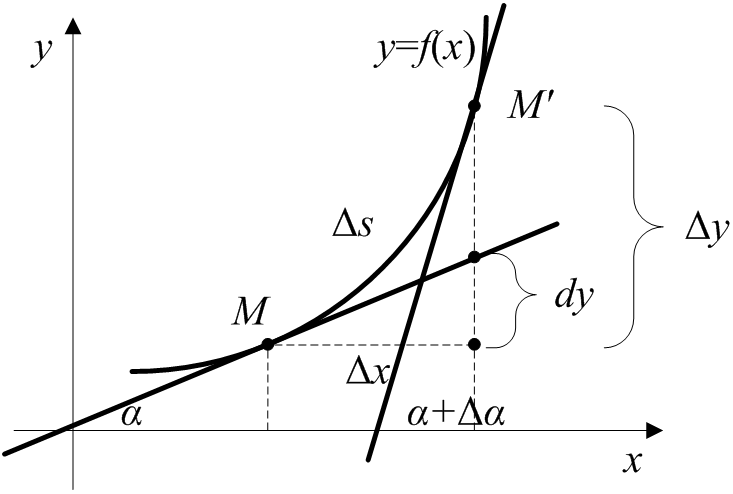
\includegraphics[height=4cm]{2.4.png}
\end{figure}

\begin{definition}[曲率]
我们定义曲线$y$上,切线转过的角度$\Delta \alpha $和弧长$\Delta s=\overset\frown{MM'}$的比值为{\bf 该弧段的平均曲率},记作$\bar{\kappa}$,即:
\[
\bar{\kappa}:=\frac{\Delta \alpha}{\Delta s}
\]
如果当$\Delta s\rightarrow 0$时$\bar{\kappa}$存在极限,就称该极限为{\bf 曲线$y$在点{\it M}处的曲率},记作$\kappa $,即:
\[
\kappa :=\underset{\Delta s\rightarrow 0}{\lim}\bar{\kappa}=\underset{\Delta s\rightarrow 0}{\lim}\frac{\Delta \alpha}{\Delta s}=\frac{d\alpha}{ds}
\]
\end{definition}

首先求解$d\alpha $:
\begin{align*}
&\because \frac{dy}{dx}=\tan \alpha \\
&\therefore \frac{d^2y}{dx^2}=\frac{d}{dx}\left( \tan \alpha \right) =\sec ^2\alpha \cdot \frac{d\alpha}{dx} \\
&\therefore d\alpha =\frac{d^2y}{dx^2}\cdot \frac{dx}{\sec ^2\alpha}=\frac{d^2y}{dx^2}\cdot \frac{dx}{1+\tan ^2\alpha}=\frac{d^2y}{dx^2}\cdot \frac{1}{1+\left( \frac{dy}{dx} \right) ^2}\cdot dx
\end{align*}
再求解$ds$(称为{\bf 弧微分}):
\[
ds=\sqrt{\left( dx \right) ^2+\left( dy \right) ^2}=\sqrt{1+\left( \frac{dy}{dx} \right) ^2}\cdot dx
\]
结合上述两式,得到曲率公式:
\[
\kappa =\underset{\Delta s\rightarrow 0}{\lim}\bar{\kappa}=\underset{\Delta s\rightarrow 0}{\lim}\frac{\Delta \alpha}{\Delta s}=\frac{d\alpha}{ds}=\frac{\frac{d^2y}{dx^2}\cdot \frac{1}{1+\left( \frac{dy}{dx} \right) ^2}\cdot dx}{\sqrt{1+\left( \frac{dy}{dx} \right) ^2}\cdot dx}=\frac{d^2y}{dx^2}\cdot \frac{1}{\left[ 1+\left( \frac{dy}{dx} \right) ^2 \right] ^{3/2}}
\]

\begin{tcolorbox}
曲率有正有负,表示凸还是凹。
其次,弧微分这个概念在微积分中会频繁出现,特别是在多元函数微积分中。
\end{tcolorbox}






\newpage
\section{本章小结}

形而下来讲,本章引入了微积分里的灵魂概念——导数。
如果将微积分定位为工程上的数学工具,则导数是这个工具中的数学基础,微分是作为数学的导数的第一个工程应用,如何用一个微小量代替全部量。
形而上来讲,本章解决了光滑的第二个要求。
至此,光滑的好函数——不断不折——在数学上有了严格的定义。

我们要将“光滑”这个概念作为微积分的出发点和落脚点,深入理解极限、连续、导数、微分这些概念。
我们喜欢的是光滑曲线,我们要考察的是光滑曲线,我们要寻找使用的也是光滑曲线。
所以我们首先定义光滑——不断不折。
通过连续定义什么是不断,通过可导定义什么是不折。
接着,我们考察光滑曲线的特征。
光滑的特征体现在连续上是最值、有界、介值三个定理。
由于可导等价于可微,所以不折的特征体现在可导上是微分中值定理,特别是拉格朗日定理。
充分领悟光滑这个概念,这些定理将会是无比自然。
最后,我们从“微”的角度考察光滑的好处,即光滑的实际价值。
我们提出了微分的概念,用一个线性小量代替绝对差量,当然,这得首先要求是光滑的。

至此,我们解决了光滑的问题,讨论了光滑在“微”方面的意义。
下一章积分,我们要讨论光滑在“累积”方面有哪些特征,可以帮助我们解决什么问题。






\newpage
\section{习题}

\begin{exercise}
求曲线$y=\cos x$在点$\left( \frac{\pi}{3},\frac{1}{2} \right) $处的切线和法线方程。
\end{exercise}

解:

使用曲线的切线和法线的公式即可。
\begin{align*}
&y=f'\left( x_0 \right) x+\left[ f\left( x_0 \right) -f'\left( x_0 \right) x_0 \right] \\
&y=-\frac{1}{f'\left( x_0 \right)}x+\left[ f\left( x_0 \right) +\frac{1}{f'\left( x_0 \right)}x_0 \right]
\end{align*}
得到切线和法线方程:
\begin{align*}
&\because f'\left( \frac{\pi}{3} \right) =-\sin \left( \frac{\pi}{3} \right) =-\frac{\sqrt{3}}{2} \\
&\therefore \begin{cases}
	y=-\frac{\sqrt{3}}{2}x+\left( \frac{1}{2}+\frac{\sqrt{3}}{2}\frac{\pi}{3} \right)\\
	y=\frac{1}{\frac{\sqrt{3}}{2}}x+\left( \frac{1}{2}+\frac{1}{-\frac{\sqrt{3}}{2}}\frac{\pi}{3} \right) =\frac{2}{\sqrt{3}}x+\left( \frac{1}{2}-\frac{2}{\sqrt{3}}\frac{\pi}{3} \right)\\
\end{cases}
\end{align*}

~

\begin{exercise}
求曲线$e^{xy}-2x-y=3$上点$\left( -1,0 \right) $所对应的切线方程。
\end{exercise}

解:

大体思路一样,只是需要用到隐函数求导:
\begin{align*}
&\because \frac{dy}{dx}=-\frac{F_x}{F_y}=-\frac{ye^{xy}-2}{xe^{xy}-1} \\
&\therefore f'\left( x_0 \right) =-\frac{-2}{-1-1}=-1 \\
&\therefore y=f'\left( x_0 \right) x+\left[ f\left( x_0 \right) -f'\left( x_0 \right) x_0 \right] =-x-1
\end{align*}

~

\begin{exercise}
求过点$\left( 3,0 \right) $与曲线$y=x^2$相切的直线方程。
\end{exercise}

解:

注意点$\left( 3,0 \right) $并不是曲线上的点,而是切线过的点。
假设切线切与点$x_0$,易得切线方程:
\[
y=2x_0\cdot x+\left( {x_0}^2-2x_0x_0 \right) =2x_0\cdot x-{x_0}^2
\]
带入点$\left( 3,0 \right) $求得$x_0$:
\begin{align*}
&\because 0=6x_0-{x_0}^2 \\
&\therefore x_0=0\,\,\mathrm{or}\,\,6
\end{align*}
于是得到2条切线:
\begin{align*}
&y=0 \\
&y=12x-36
\end{align*}

~

\begin{exercise}
在抛物线$y=1-x^2$上求两点,使得过这两点的切线与{\it x}轴形成一个等边三角形。
\end{exercise}

解:

首先假设切点为$x_0$,获得切线方程:
\[
y=\left( -2x_0 \right) x+\left[ \left( 1-{x_0}^2 \right) -\left( -2x_0 \right) x_0 \right] =\left( -2x_0 \right) x+\left( 1+{x_0}^2 \right)
\]
若与{\it x}轴形成等边三角形,则这两条直线的斜率必为$\pm \sqrt{3}$,于是:
\begin{align*}
&\because -2x_0=\pm \sqrt{3}\Rightarrow x_0=\pm \frac{\sqrt{3}}{2} \\
&\therefore \left( \pm \frac{\sqrt{3}}{2},\frac{1}{4} \right)
\end{align*}

~

\begin{exercise}
求和$y=x^2,y=-x^2+6x-5$两条曲线都相切的直线方程。
\end{exercise}

解:

假设和两条曲线分别切于点$x_1,x_2$,分别根据两条曲线易得切线:
\begin{align*}
y&=2x_1x+\left( {x_1}^2-2x_1x_1 \right) =2x_1x-{x_1}^2 \\
y&=\left( -2x_2+6 \right) x+\left[ \left( -{x_2}^2+6x_2-5 \right) -\left( -2x_2+6 \right) x_2 \right] \\
&=\left( -2x_2+6 \right) x+\left( {x_2}^2-5 \right)
\end{align*}
由于这两条切线是同一条,于是可以得到:
\[
\begin{cases}
	2x_1=-2x_2+6\\
	-{x_1}^2={x_2}^2-5\\
\end{cases}\Rightarrow \begin{cases}
	x_1=1\\
	x_2=2\\
\end{cases} \quad \mathrm{or} \quad \begin{cases}
	x_1=2\\
	x_2=1\\
\end{cases}
\]
即有两条切线都可以和$y=x^2,y=-x^2+6x-5$相切:
\begin{align*}
&y=2x-1 \\
&y=4x-4
\end{align*}

~

\begin{exercise}
给定椭圆$4x^2+y^2=5$,求与此椭圆相切于$\left( \pm 1,-1 \right) $的抛物线方程。
\end{exercise}

解:

椭圆和抛物线相切,则必有一切线,同时切于这两个曲线。
先求和椭圆的切于$\left( \pm 1,-1 \right) $的切线方程,椭圆方程的隐函数为$F=4x^2+y^2-5$,则切线:
\begin{align*}
&\because y'\left( x_0 \right) =-\frac{F_x}{F_y}=-\frac{8x_0}{2y_0} \\
&\therefore y=f'\left( x_0 \right) x+\left[ f\left( x_0 \right) -f'\left( x_0 \right) x_0 \right] =-\frac{8x_0}{2y_0}x+\left[ y_0+\frac{8x_0}{2y_0}x_0 \right] \\
&\therefore \begin{cases}
	y=-\frac{8x_0}{2y_0}x+\left[ y_0+\frac{8x_0}{2y_0}x_0 \right] =4x-5\\
	y=-\frac{8x_0}{2y_0}x+\left[ y_0+\frac{8x_0}{2y_0}x_0 \right] =-4x-5\\
\end{cases}
\end{align*}
假设抛物线方程$y=ax^2+bx+c$,则有切线:
\begin{align*}
&\because y'\left( x_0 \right) =2ax_0+b \\
&\therefore y=f'\left( x_0 \right) x+\left[ f\left( x_0 \right) -f'\left( x_0 \right) x_0 \right] =\left( 2ax_0+b \right) x+\left[ y_0-\left( 2ax_0+b \right) x_0 \right] \\
&\therefore \left\{ \begin{aligned}
	y&=\left( 2ax_0+b \right) x+\left[ y_0-\left( 2ax_0+b \right) x_0 \right]\\
	&=\left( 2a+b \right) x+\left[ -1-\left( 2a+b \right) \right]\\
	y&=\left( 2ax_0+b \right) x+\left[ y_0-\left( 2ax_0+b \right) x_0 \right]\\
	&=\left( -2a+b \right) x+\left[ -1+\left( -2a+b \right) x_0 \right]\\
\end{aligned} \right.
\end{align*}
于是得到:
\[
\begin{cases}
	2a+b=4\\
	-1-\left( 2a+b \right) =-5\\
	-2a+b=-4\\
	-1+\left( -2a+b \right) =-5\\
\end{cases}
\]
解得$a=2,b=0$后得到抛物线方程$y=2x^2+c$,再将$\left( \pm 1,-1 \right) $代入求得$c=-3$,于是最终得到抛物线方程:
\[
y=2x^2-3
\]

~

\begin{exercise}
若$f\left( x \right) $对任意实数$x_1,x_2$有$f\left( x_1+x_2 \right) =f\left( x_1 \right) f\left( x_2 \right) $,且$f'\left( 0 \right) =1$,证明$f'\left( x \right) =f\left( x \right) $。
\end{exercise}

解:

总体思路求解$f'\left( x \right) $。

首先我们可以根据$f\left( x_1+x_2 \right) =f\left( x_1 \right) f\left( x_2 \right) $得到:
\begin{align*}
&\because f\left( x_1+x_2 \right) =f\left( x_1 \right) f\left( x_2 \right) \\
&\therefore f\left( x \right) =f\left( 0 \right) f\left( x \right) \\
&\therefore f\left( 0 \right) =0\,\,\mathrm{or}\,\,1
\end{align*}
其次,将$f\left( x_1+x_2 \right) =f\left( x_1 \right) f\left( x_2 \right) $两边求导得到:
\begin{align*}
&\because f'\left( x_1+x_2 \right) =\left[ f\left( x_1 \right) f\left( x_2 \right) \right] '=f'\left( x_1 \right) f\left( x_2 \right) +f\left( x_1 \right) f'\left( x_2 \right) \\
&\therefore f'\left( x \right) =f'\left( x+0 \right) =f'\left( x \right) f\left( 0 \right) +f\left( x \right) f'\left( 0 \right) =f'\left( x \right) f\left( 0 \right) +f\left( x \right)
\end{align*}
当$f\left( 0 \right) =0$时,有
\[
f'\left( x \right) =f'\left( x \right) f\left( 0 \right) +f\left( x \right) =f\left( x \right)
\]
当$f\left( 0 \right) =1$时,有
\[
f'\left( x \right) =f'\left( x \right) f\left( 0 \right) +f\left( x \right) =f'\left( x \right) +f\left( x \right)
\]
此时解得函数表达式为$f\left( x \right) =0$,也即$f'\left( x \right) =f\left( x \right) $,证毕。









